\documentclass[aspectratio=43]{beamer}
\usepackage[version=4]{mhchem}
\usepackage[aboveskip=1pt, belowskip=1pt]{caption}
\usepackage{amsmath}
\usepackage{siunitx}

% Command to display isotopes
\newcommand{\iso}[2]{\ce{^{#1}#2}}
% Set caption package options
\captionsetup{labelformat=empty}

\title[SF quenching]{Quenching of spectroscopic factors in \\ \texorpdfstring{\iso{10,12}{Be}(d, \iso{3}{He})}{10,12Be(d,3He)} reactions}
\date{Zakopane 2024 Conference}
\author[M. Lozano et al.]{M. Lozano-González, A. Matta, B. Fernández-Domínguez}
\institute{IGFAE and LPC-Caen}

\usetheme{igfae}

\begin{document}

\maketitle

\section{Motivation}
\begin{frame}{A recap on spectroscopic factors}
    \textbf{Spectroscopic factors} shed light on the occupancy of single-particle states:
    \begin{equation*}
        \left.\frac{d\sigma}{d\Omega}\right\vert_{exp} = C^{2}S \cdot \left.\frac{d\sigma}{d\Omega}\right\vert_{s.p}, \quad C^{2}S = (2j + 1) \text{ or } 1 \text{ in IPSM}
    \end{equation*}
    \begin{columns}[T]
        \begin{column}{0.48\linewidth}
            \hfill{}
            \begin{beamercolorbox}[sep=0.75em, center, wd=0.85\linewidth,rounded=true]{box1}
                \textbf{Experimentally:} Reduction of \sim\qty{65}{\percent}!
            \end{beamercolorbox}%
            \hfill{}
            \begin{itemize}
                \item \textbf{Long-range} correlations: vibrations, giant resonances,...
                \item \textbf{Short-range}: tensor forces,...
            \end{itemize}
        \end{column}
        \begin{column}{0.48\linewidth}
            \begin{figure}
                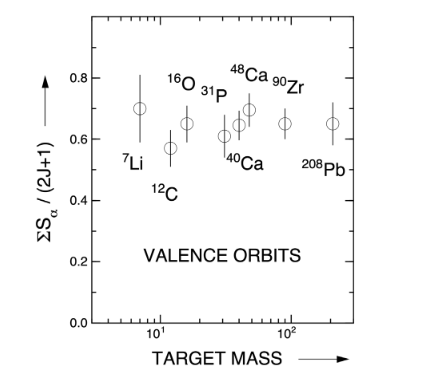
\includegraphics[width=0.9\linewidth]{figures/SF_aumann_review.png}
                \caption{L. Lapikás, Nuclear Phys. A 553 (1993)}
            \end{figure}
        \end{column}
    \end{columns}
\end{frame}

\begin{frame}{A long-standing puzzle}
    A trend with asymmetry energy $\Delta S \equiv S_{n} - S_{p}$ is found depending on the experimental \textbf{probe}!
    \begin{figure}
        \begin{tikzpicture}
            \node[anchor=south west,inner sep=0] (image) at (0,0) { 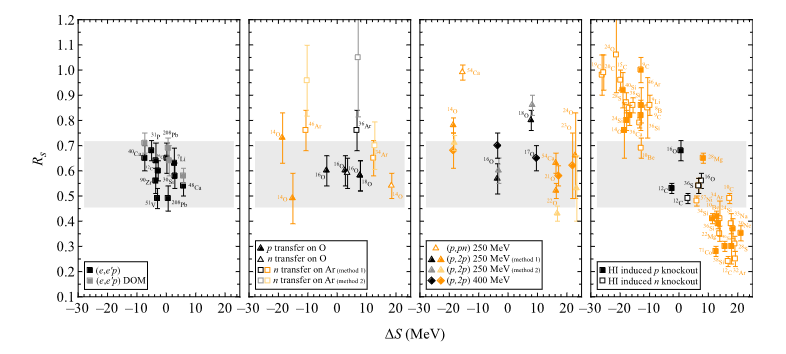
\includegraphics[width=0.9\linewidth]{figures/Rs_aumann_review.png}
            };
            \myscope{
                \node at (0.2, 0.85) {(e, e'p)};
                \node at (0.42, 0.85) {transfer};
                \node at (0.63, 0.85) {(p,2p)};
                \node[align=center] at (0.85, 0.85) {\textcolor{red}{Be-C} \\ \textcolor{red}{knock-out}};
                \draw[thick, red] (0.8, 0.7) -- (0.93, 0.32);
            }
        \end{tikzpicture}
        \caption{T. Aumann \textit{et al.} Prog. Part. Nucl. Phys. 118 (2021)}
    \end{figure}
    \mycolorbox{box2}{
        $\Rightarrow$ measure towards more exotic nuclei: $\left|\Delta S \right| \uparrow$
    }
\end{frame}

\begin{frame}[t]{Status with light isotopes}
    Several experiments allowed for the extraction of $C^{2}S$ with Li-induced (d, \iso{3}{He}) reactions:
    \vspace{-1.75em}
    \begin{columns}[c]
        \column{0.48\linewidth}{
            \begin{tikzpicture}
                \node[anchor=south west, inner sep=0](image) at (0,0){
                    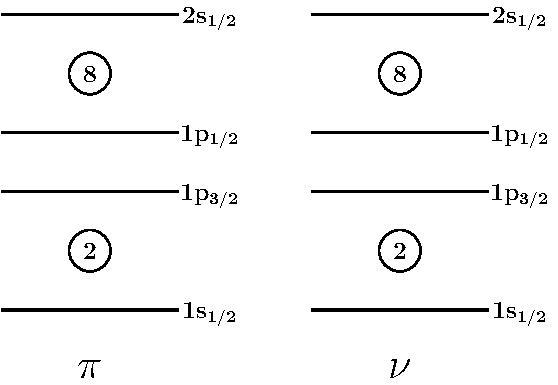
\includegraphics[width=0.75\linewidth]{figures/empty_shell_model.pdf}
                };
                \myscope[false]{
                \node[rectangle, draw, thick, magenta, fit={(0.0, 0.7)(0.4,0.5)},
                label={[align=center]west:{\small This\\ \small region}}] at (0.2, 0.55) {};
                }
            \end{tikzpicture}
        }%
        \column{0.48\linewidth}{
            \begin{figure}
                \begin{tikzpicture}
                    \node[anchor=south west, inner sep=0](image) at (0,0){
                        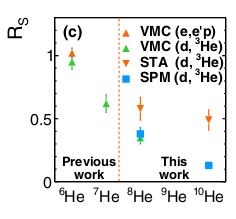
\includegraphics[width=0.75\linewidth]{figures/matta_Rs_Li_He.png}
                    };
                    \myscope[false]{
                    \node[rectangle, draw, very thick, magenta, fit={(0.9, 0.1)(0.8, 0.2)},pin={
                    [pin distance=7mm,
                            pin edge={<-, very thick, black}]75:{\small \color{red} Unbound!}}
                    ] at (0.9, 0.1) {};
                    }
                \end{tikzpicture}
                \caption{A. Matta \textit{et al.}, Phys. Rev. C 92 (2015)}
            \end{figure}
        }
    \end{columns}
    Several challenges in this region:
    \begin{columns}[T]
        \begin{column}{0.48\linewidth}
            \begin{itemize}
                \item Dealing with \textbf{unbound} nuclei (\iso{10}{Be})
            \end{itemize}
        \end{column}
        \begin{column}{0.48\linewidth}
            \begin{itemize}
                \item Impact of core exitations (completar algo +)
            \end{itemize}
        \end{column}
        % \column{0.28\linewidth}{
        % \mycolorbox{box3}{
        % $R_{s} \equiv \frac{C^2S_{\text{exp}}}{C^{2}S_{\text{theo}}}$
        % }
        % }
        % \column{0.68\linewidth}{
        %     \begin{itemize}
        %         \item Unbound nuclei (\iso{10}{He}) $\Rightarrow$ move to the Li chain: \iso{11}{Li} is weakly bound.
        %         \item Other physics beyond quenching: \textbf{geometrical} mismatch factor
        %     \end{itemize}
        % }
    \end{columns}

\end{frame}

\begin{frame}[t]{Importance of GMF}
    Towards exotic nuclei (loosely bound or halo), a \textbf{\textit{geometrical mismatch factor}} emerges from the very different w.f. in the overlap:
    \vspace{-1em}
    \begin{columns}[T]
        \column{0.48\linewidth}
        {
            \begin{figure}
                \begin{tikzpicture}
                    \node[anchor=south west, inner sep=0pt] (image) at (0,0){
                        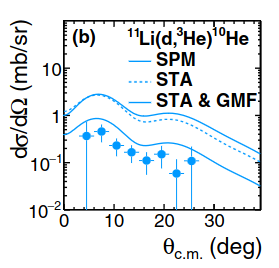
\includegraphics[width=0.7\linewidth]{figures/matta_11Li_d3He.png}};
                    \myscope[false]{
                        \draw[<-, very thick, magenta] (0.6, 0.46) -- (0.68, 0.54);
                        \draw[<-, very thick, magenta] (0.3, 0.55) -- (0.35, 0.65);
                    }
                \end{tikzpicture}
                \caption{A.Matta et al., Phys. Rev. C 92 (2015)}
            \end{figure}
        }
        \column{0.48\linewidth}
        {
            \begin{figure}
                \begin{tikzpicture}
                    \node[anchor=south west, inner sep=0pt] (image) at (0, 0){
                        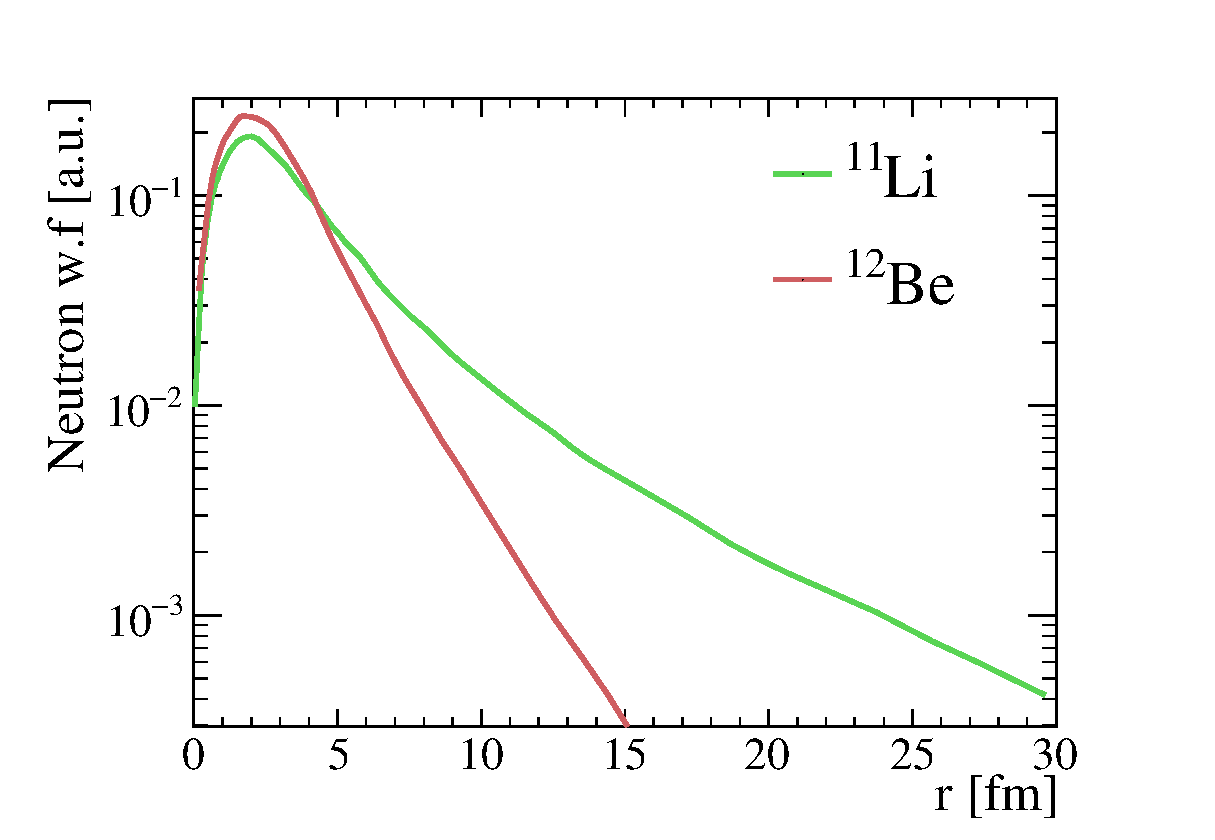
\includegraphics[width=1\linewidth]{figures/wfs.eps}};
                    \myscope[false]{
                        \draw[<->, very thick, dashed, magenta] (0.47, 0.25) -- (0.7, 0.25);
                    }
                \end{tikzpicture}
                \caption{N. K. Timofeyuk, private communication (in E748 proposal)}
            \end{figure}
        }
    \end{columns}
    \begin{columns}[c]
        \begin{column}{0.78\linewidth}
            \mycolorbox[1]{box4}{
                $\Rightarrow$ Need to establish more systematics for this parameter
            }
        \end{column}
    \end{columns}
    % \begin{column}{0.5\linewidth}
    %     \mycolorbox[0.95]{box4}{
    %         \begin{itemize}
    %             \item Measure $\left\langle\iso{10,12}{Be}\middle|\iso{9,11}{Li}\right\rangle$
    %             \item $\Delta S = -12.8 | -19.8 \unit{\MeV}$
    %         \end{itemize}
    %     }
    % \end{column}%
    % \begin{column}{0.5\linewidth}
    %     \mycolorbox{box1}{
    %         \begin{itemize}
    %             \item Establish systematics for \textbf{\color{magenta} GMF}
    %         \end{itemize}
    %     }
    % \end{column}
    % \end{columns}
\end{frame}

\begin{frame}{Physics case of E748}
    E748 @ GANIL back in 2017. Using \iso{10,12}{Be}(d,\iso{3}{He}) reactions to:
    \bigskip
    \begin{columns}[T]
        \begin{column}{0.52\linewidth}
            \mycolorbox[1]{box2}{
            Overlaps:
            {\small
            \begin{itemize}
                \item $\left\langle\iso{10}{Be}\middle|\iso{9}{Li}\right\rangle, \Delta S = \qty{-12.8}{\MeV}$
                \item $\left\langle\iso{12}{Be}\middle|\iso{11}{Li}\right\rangle, \Delta S = \textcolor{magenta}{\qty{-19.8}{\MeV}}$
            \end{itemize}}
            \begin{tikzpicture}
                \node[anchor=south west, inner sep = 0pt] (image) at(0, 0){
                    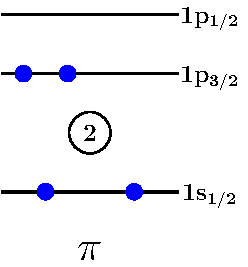
\includegraphics[width=0.6\linewidth]{figures/Be_proton_shell_model.pdf}
                };
                \myscope[false]{
                \node[pin={[pin distance=8mm, pin edge={<-, very thick, magenta}]-95:{\footnotesize This strength}}] at (0.3, 0.7) {};
                }
            \end{tikzpicture}
            }
        \end{column}
        \begin{column}{0.48\linewidth}
            \mycolorbox[1]{box3}{\small
                Explore effects of GMF:
                \begin{itemize}
                    \item $\left\langle\iso{10}{Be}\middle|\iso{9}{Li}\right\rangle, \text{GMF} \sim \num{1}$
                    \item $\left\langle\iso{12}{Be}\middle|\iso{11}{Li}\right\rangle, \text{GMF} \sim \textcolor{blue}{\num{0.5}?}$
                \end{itemize}
                \begin{tikzpicture}[scale=0.8]
                    \datavisualization [
                        scientific axes,
                        visualize as line/.list={be,li},
                        be={pin in data={text=Be, when=x is 1.5, pin length=2ex}},
                        li={pin in data={text=Li, when=x is 1.5, pin length=2ex}},
                        % li={label in legend={text=Li}},
                        style sheet=strong colors,
                        x axis={include value=-1, include value=2,
                                ticks={major at={
                                                0 as $\langle\iso{10}{Be}\vert\iso{9}{Li}\rangle$,
                                                1 as $\langle\iso{12}{Be}\vert\iso{11}{Li}\rangle$
                                            }}},
                        y axis={label={$S_{n}$ [MeV]}, include value=0, include value=8}]
                    data [set=be,format=TeX code]{
                            \pgfkeys{/data point/.cd,x=0, y=6.8} \pgfdatapoint
                            \pgfkeys{/data point/.cd,x=1, y=3.2} \pgfdatapoint
                        }
                    data [set=li,format=TeX code]{
                            \pgfkeys{/data point/.cd,x=0, y=4.1} \pgfdatapoint
                            \pgfkeys{/data point/.cd,x=1, y=0.4} \pgfdatapoint
                        };
                \end{tikzpicture}
            }
        \end{column}
    \end{columns}
\end{frame}

\section{Methodology}
\begin{frame}[c]{Experimental setup}
    Tradional solid target experiment @ LISE
    \vspace{1.5em}
    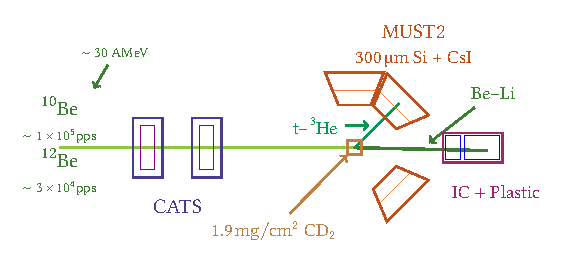
\includegraphics[width=1\linewidth]{figures/setup.pdf}
\end{frame}
\end{document}